\documentclass{bilidoc}

\title{\textbf{\href{http://dx.doi.org/10.3208/sandf1972.14.3_1}{Shear Modulus and Shear Strength of Cohesive Soils}\\黏性土的剪切模量和剪切强度}}
\date{\today}
\author{Akio Hara \and Tokiharu Ohta \and Masanori Niwa \and Shumpei Tanaka \and Tadashi Banno}

\renewcommand{\theenumi}{\arabic{enumi}}
\renewcommand{\labelenumi}{(\theenumi)}

\begin{document}

\maketitle

\section*{Abstract 摘要}

\begin{paracol}{2}

    The purpose of this paper is to evaluate the relation between initial shear modulus and shear strength of cohesive soils. The initial shear moduli were obtained from the results of the well-shooting tests by means of shear waves, while the shear strength could be obtained from the results of laboratory tests conducted on undisturbed soil samples collected at the same site as the well-shooting tests. Taking into consideration the fact that there have been a number of instances where the well-shooting test and the standard penetration test were conducted on the same sites, the authors conducted their research to seek some relationships between the initial shear modulus and the N-value of the standard penetration test, between the shear strength and the N-value, and between the initial shear modulus and the shear strength. The research works have finally led the authors to finding out several relations among initial shear modulus, shear strength and N-value.

    \textbf{Key words: }cohesive soil, elasticity, geophysical exploration, in-situ test, laboratory test, penetration test, shear strength.

    \switchcolumn

    本文的目的是评估黏性土的初始剪切模量与剪切强度之间的关系。 初始剪切模量是通过剪切波从地震测井试验的结果中获得的,而抗剪强度可以从对与地震测井试验在同一地点采集的未扰动土体样品进行的实验室试验结果中获得。 考虑到在许多情况下都在同一地点进行了地震测井试验和标准贯入试验,因此作者进行了研究,以寻求初始剪切模量与标准贯入试验的N值之间,剪切强度与N值之间以及初始剪切模量与剪切强度之间的一些关系。 研究工作最终使作者找到了初始剪切模量,剪切强度和N值之间的几种关系。

    \textbf{关键词:}黏性土,弹性,地球物理勘探,原位试验,实验室试验, 贯入试验,剪切强度。

\end{paracol}

\section{INTRODUCTION 介绍}

\begin{paracol}{2}

    In Japanese cities, for lack of suitable building sites, there has recently been a marked tendency to plan construction of large and tall buildings on soft grounds which were never considered in the past as a building site. Every structure is influenced by the local ground behavior to a considerable extent during earthquakes, especially when built on a soft ground. Since any structure built on such a ground is inevitably subject to considerable displacement, particularly at its foundation, it is desirable that an earthquake-proof design follows a dynamic analysis by means of a simulation model of structure-foundation-ground system. Needless to mention, understanding by experiment of the dynamic properties of soils is required for such a dynamic analysis. These properties are characterized by the following items:
    \begin{enumerate}
        \item Initial shear modulus
        \item Shear strength
        \item Non-linear characteristics
        \item Damping
    \end{enumerate}

    \switchcolumn

    在日本城市中,由于缺乏合适的建筑工地,最近有一种明显的趋势是计划在柔软的地面上建造大型高层建筑,而过去从未将其视为建筑工地。 在地震期间,尤其是在软土地上建造时,每个结构在很大程度上都会受到当地地面行为的影响。 由于在这样的地面上建造的任何建筑物都不可避免地会遭受相当大的位移,特别是在其基础上,因此希望通过结构基础-地面系统的仿真模型对动态设计进行抗震设计。 不用说,进行这种动力学分析需要通过实验来了解土壤的动力学特性。 这些特性的特征如下:
    \begin{enumerate}
        \item 初始剪切模量
        \item 剪切强度
        \item 非线性特性
        \item 阻尼
    \end{enumerate}

    \switchcolumn*

    In order to research the above problems, it is desirable to make the best of the merits of the in-situ test and the laboratory test. By in-situ tests we are able to grasp directly the mechanical properties of soils at natural soil deposit, but the test conditions are not always clear.On the other hand, conditions of the laboratory test are clear, and the laboratory test enables us to obtain the mechanical properties at large deformation, but its weak point is disturbance of soil structure during the sampling and testing processes.
    
    Therefore the in-situ and the laboratory tests have their merits and demerits. In order to take advantage of the merits, the authors took notice of the following items : 

    \switchcolumn

    为了研究上述问题,希望充分利用原位试验和实验室试验的优点。 通过现场试验,我们能够直接掌握天然土壤沉积物的土壤力学性能,但是试验条件并不总是很清楚。另一方面,实验室试验的条件是明确的,并且实验室试验使我们能够获得大变形时的机械性能,但是它的弱点是在采样和试验过程中对土壤结构的干扰。
  
    因此,现场试验和实验室试验各有优缺点。 为了利用这些优点,作者注意到以下几点:

    \switchcolumn*

    \begin{enumerate}
        \item There are many cases where soil stiffness increases in general with strength according to the experience of laboratory or in-situ test.
        \item \citet{Wilson2010419} presented many data on Young's modulus E and undrained shear strength Su by the laboratory test. Furthermore, \citet{DAppolonia19711359} showed a number of data on Young's modulus $E$ obtained from initial settlement curve and undrained shear strength $S_u$. It is recognized that the values of ratio $E/S_u$ calculated from their data are within a certain limited region.
        \item The shear strength of soil can be calculated from the values of effective overburden pressure, angle of internal friction and cohesion, and the angle of internal friction depends upon the value of plasticity index, that is, it is affected by a number of factors. Furthermore, both dimensions of initial shear modulus and of shear strength are same. It is not without reason, therefore, to consider that initial shear modulus is closely related to shear strength.
    \end{enumerate}

    \switchcolumn

    \begin{enumerate}
        \item 根据实验室或现场试验的经验,在许多情况下,土壤刚度通常随强度而增加。
        \item \citet{Wilson2010419}通过实验室试验提供了许多有关杨氏模量$E$和不排水剪切强度$S_u$的数据。 此外,\citet{DAppolonia19711359}还从大量初始沉降曲线和不排水抗剪强度$S_u$获得的杨氏模量$E$的数据。 可以认识到,根据它们的数据计算出的比率$E/S_u$的值在一定范围内。
        \item 土的抗剪强度可以根据有效上覆压力,内摩擦角和内聚力的值来计算,内摩擦角取决于可塑性指数的值,即受多种因素影响。 此外,初始剪切模量和剪切强度的尺寸都相同。 因此,并非没有理由考虑初始剪切模量与剪切强度密切相关。
    \end{enumerate}

    \switchcolumn*
    
    The authors have tried, from the above mentioned reasons, to review the relation between initial shear modulus and shear strength of cohesive soils on the basis of the results of their own in-situ test (well-shooting test, standard penetration test) and laboratory test (triaxial compression test).

    \switchcolumn

    基于上述原因,作者试图根据他们自己的现场试验(射井试验,标准渗透试验)和实验室试验(三轴压缩试验)的结果来回顾粘性土的初始剪切模量与剪切强度之间的关系。


\end{paracol}
\section{INITIAL SHEAR MODULUS OF SOILS 土的初始剪切模量}

\Paragraph{Well-Shooting Method  地震测井试验}

\begin{paracol}{2}
    
    \citet{Miller1972545}  show that the geophysical exploration test comprises several types of practical methods (cross-hole, down-hole, up-hole, surface refraction and surface-vibration mothods).
    
    The down-hole method is to generate shear waves by hitting horizontally a wooden plate placed on the ground surface, so that velocity transducers clamped in a borehole receive such shear waves. To say more precisely, several velocity transducers are concurrently clamped in the borehole, which allow velocity measurement of a shear wave passing through a section ·between one transducer and the another.
    
    When the shear wave velocity $V_s$ is measured, shear modulus $G$ can be calculated by the following equation :

    \switchcolumn

    \citet{Miller1972545}表明,地球物理勘探试验包含几种类型的实用方法:横孔,井下,井上,表面折射和表面振动方法。
    
    井下方法是通过水平击打放置在地面上的木板来产生剪切波,以便夹在井眼中的速度传感器接收这些剪切波。 更准确地说,是将多个速度传感器同时夹紧在钻孔中,从而可以测量穿过一个传感器与另一个传感器之间的截面的剪切波的速度。
    
    当测量剪切波速度$V_s$时,剪切模量$G$可以通过以下公式计算:

\end{paracol}
    
\begin{align}
    G=\rho{}V_s^2(\rm{kg/cm^2})
    \label{equation:1}
\end{align}

\begin{paracol}{2}
    \noindent where $\rho$: mass density.

    This is the procedure called the well-shooting test by means of shear waves, on which \citet{Kitsunezaki19671,Shima19681301, Shima1969819, Imai197017} have already published their respective reseach papers.

    \switchcolumn

    \noindent 式中$\rho$:质量密度。

    这就是通过剪切波进行的所谓的地震测井试验程序,\citet{Kitsunezaki19671,Shima19681301, Shima1969819, Imai197017}已经在此上发表了各自的研究论文。

\end{paracol}

\Paragraph{Shear Strain Amplitude in Soil Deposits 土壤沉积物中的剪切应变幅值}

\begin{paracol}{2}
    
    Initial shear modulus can be defined as shear modulus at infinitely small shear strain amplitude.
    
    It is therefore necessary to obtain shear strain amplitude in soil deposits when the wellshooting test by means of shear waves is to be conducted.
    
    The reslt of the well-shooting test which was performed in a soft clay deposit, as an example, is shown in \autoref{figure:1}. The authors tried to calculate shear strain amplitude in a soft soil deposit from wave forms shown in \autoref{figure:1} with the following procedure: 

    \switchcolumn

    初始剪切模量可以定义为无限小剪切应变幅值下的剪切模量。
    
    因此,当要通过剪切波进行地震测井试验时,有必要获得土壤沉积物中的剪切应变振幅。
            
    例如,在软黏土矿床中进行的地震测井试验的结果如\cnfigureref{figure:1}所示。作者试图通过\cnfigureref{figure:1}所示的波形计算软土矿床中的剪切应变幅值,其中 步骤如下:

\end{paracol}


\begin{figure*}[!htb]
    \begin{minipage}[t]{0.66\textwidth}
        \centering
        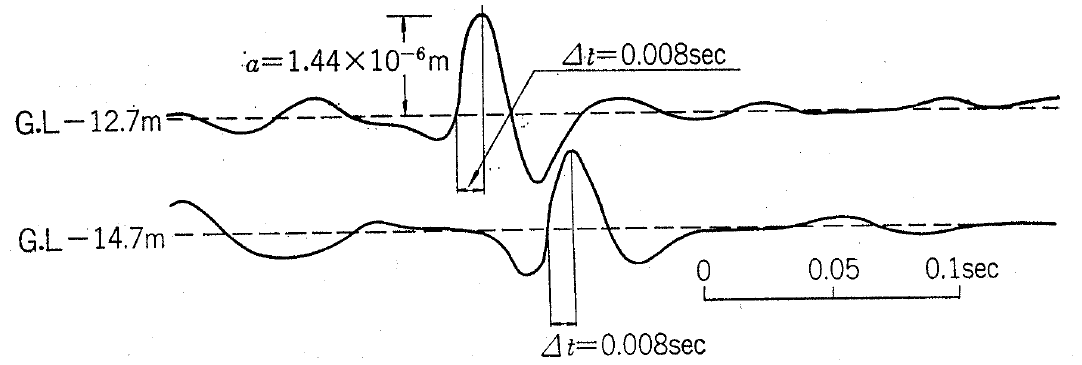
\includegraphics[width=\textwidth]{figures/figure-1.png}
        \caption{An example of shear wave velocity measurement}
        \addtocounter{figure}{-1}
        \vspace{-5pt}
        \renewcommand{\figurename}{图}
        \caption{剪切波速度测量示例}
        \renewcommand{\figurename}{Figure}
        \label{figure:1}
    \end{minipage}
    \begin{minipage}[t]{0.32\textwidth}
        \centering
        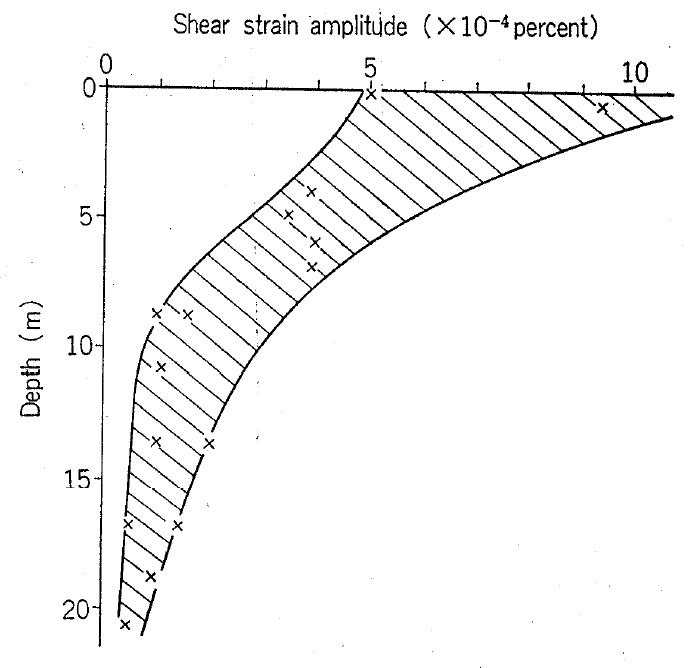
\includegraphics[width=\textwidth]{figures/figure-2.png}
        \caption{Estimated shear strain·amplitude at various depths}
        \addtocounter{figure}{-1}
        \vspace{-5pt}
        \renewcommand{\figurename}{图}
        \caption{各种深度的估计剪切应变振幅}
        \renewcommand{\figurename}{Figure}
        \label{figure:2}
    \end{minipage}
\end{figure*}


\begin{paracol}{2}
    
    (1) Calibration curves of the velocity transducers were firstly determined by shaking table in the laboratory.
    
    (2) On the assumption that principal shear wave should be represented by that of harmonic motion, the maximum shear d~splacement amplitude $\Delta{}x$ was estimated by the use of the calibration curves to be the following value:

    \switchcolumn
    
    (1)首先在实验室中通过振动台确定速度传感器的校准曲线。
            
    (2)假设应以谐波运动代表主剪切波,通过使用校准曲线将最大剪切位移振幅$\Delta{}x$估算为以下值:

\end{paracol}

\begin{align}
    \Delta{}x=0.0000144(\rm{m})
    \label{equation:2}
\end{align}

\begin{paracol}{2}    

    (3) On the other hand, thickness of soil deposit $\Delta{}H$ subject to shear displacement of $\Delta{}x$ can be calculated as follows :

    \switchcolumn
    
    (3)在 另一方面,受剪切位移$\Delta{}x$影响的土壤沉积物$\Delta{}H$的厚度可按以下公式计算:

\end{paracol}

\begin{align}
    \Delta{}H=V_s\cdot{}\Delta{}t=90\times{}0.008=0.72(\rm{m})
    \label{equation:3}
\end{align}

\begin{paracol}{2}

    (4) Shear strain amplitude $\gamma$ can thus be calculated as follows :

    \switchcolumn
    
    (4)因此,剪切应变幅值$\gamma$可按以下公式计算:

\end{paracol}

\begin{align}
    \gamma=\dfrac{1.44\times{}10^{-6}}{0.72}=2.0\times{}10^{-6}
    \label{equation:4}
\end{align}

\begin{paracol}{2}

    Shear strain amplitude obtained in the above procedure are plotted in \autoref{figure:2}, which shows that shear strain amplitude thus obtained by the well-shooting test can be assumed to be less than $10^{-3}\%$ percent.
    
    In addition, when shear strain amplitude is $10^{-3}\%$, shear stress as calculated below is so small that the shear modulus obtained by the well-shooting test can be regarded as initial shear modulus :

    \switchcolumn

    在上述过程中获得的剪切应变振幅绘制在\cnfigureref{figure:2}中,该曲线表明,可以将通过地震测井试验获得的剪切应变振幅假定为小于$10^{-3}\%$。
    
    另外,当剪切应变幅值为$10^{-3}\%$时,如下计算的剪切应力是如此之小,以至于通过地震测井试验获得的剪切模量可以视为初始剪切模量:

\end{paracol}

\begin{align}
    \tau=\gamma{}G=10^{-5}\times{}110=0.0011(\rm{kg/cm^2})
    \label{equation:5}
\end{align}

\Paragraph{Shear Strength of Soil 土的抗剪强度}

\begin{paracol}{2}
    
    The soil element shown in \autoref{figure:3} is deformed due to random vibrations propagating from bedrock to surface during an earthquake. In this case, the deformation excited most significantly is mainly attributable to the shear wave.

    \switchcolumn

    \cnfigureref{figure:3}所示的土壤单元由于地震期间从基岩传播到地面的随机振动而变形。 在这种情况下,最显着激发的变形主要归因于剪切波。      \switchcolumn*

    The initial stress condition of the soil element is the $K_0$-condition, which means that initial effective stresses in vertical and horizontal direction are a $\sigma_v'$ and $K_0\sigma_v'$ respectively.

    \switchcolumn
       
    土元素的初始应力条件为$K_0$条件,这意味着垂直方向和水平方向的初始有效应力为分别为$\sigma_v'$和$K_0\sigma_v'$。
    
    \switchcolumn*

    The shear modulus obtained from the well-shooting test is calculated from the velocity of the shear wave, which propagate through the soil elements vertically in the $K_0$-condition.

    \switchcolumn
       
    从地震测井试验获得的剪切模量是根据剪切波的速度计算的,剪切波的速度在$K_0$条件下垂直传播通过土体颗粒。

\end{paracol}

\begin{figure*}[!htb]
    \begin{minipage}[t]{0.54\textwidth}
        \centering
        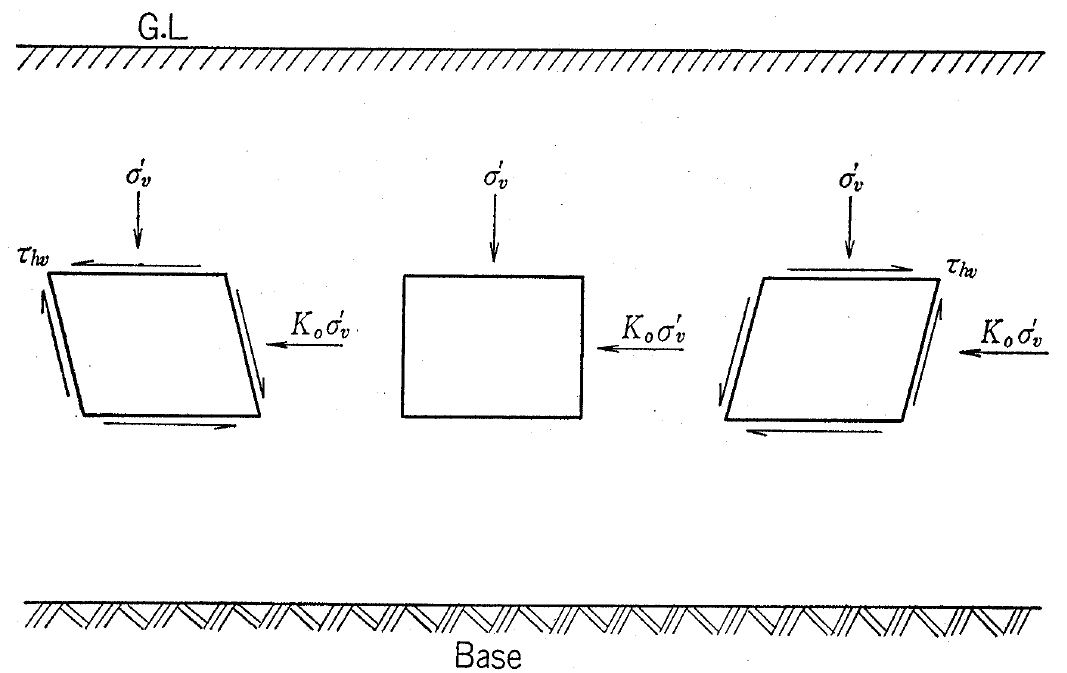
\includegraphics[width=\textwidth]{figures/figure-3.png}
        \caption{Conceptual field loading condition}
        \addtocounter{figure}{-1}
        \vspace{-5pt}
        \renewcommand{\figurename}{图}
        \caption{概念性的场地加载条件}
        \renewcommand{\figurename}{Figure}
        \label{figure:3}
    \end{minipage}
    \begin{minipage}[t]{0.42\textwidth}
        \centering
        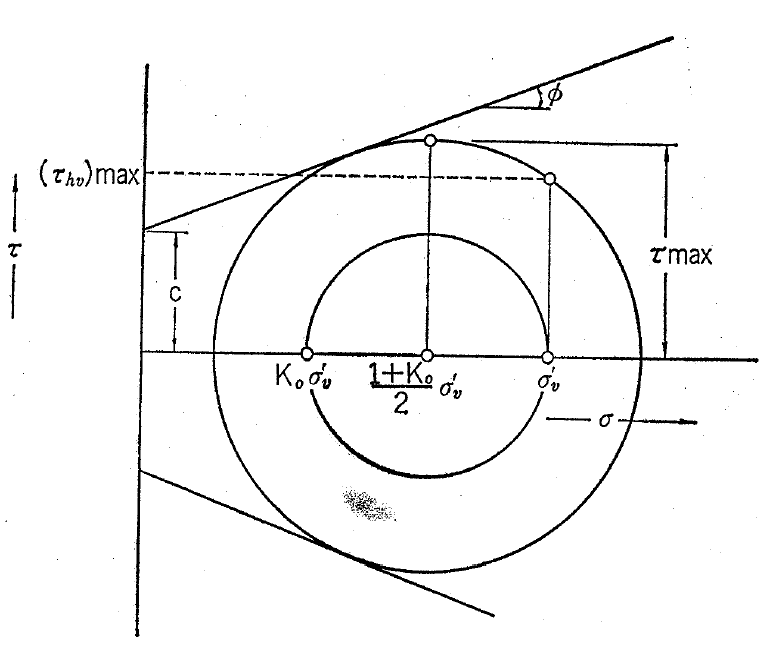
\includegraphics[width=\textwidth]{figures/figure-4.png}
        \caption{Mohr' s  circles and maximum shear stress}
        \addtocounter{figure}{-1}
        \vspace{-5pt}
        \renewcommand{\figurename}{图}
        \caption{莫尔圆和最大切应力}
        \renewcommand{\figurename}{Figure}
        \label{figure:4}
    \end{minipage}
\end{figure*}


\begin{paracol}{2}
    
    Therefore, it is reasonable that the shear strength of a soil deposit should be obtained by taking into account its initial stress condition. These problems have been sufficiently treated by Duncan, Seed and Hardin. According to these researches, when the soil element shown in \autoref{figure:3} comes to failure, the maximum lateral shear stress $(\tau_{hv})_{\rm{max}}$ is given on Mohr's circles as represented in \autoref{figure:4}. Taking the geometric relation in \autoref{figure:4} into consideration, the maximum lateral shear stress $(\tau_{hv})_{\rm{max}}$ will be

    \switchcolumn

    因此,合理的是应考虑其初始应力条件来获得土壤沉积物的剪切强度。\citet{Duncan1969101,Seed19711099,Hardin1973667}已经充分解决了这些问题。 根据这些研究,当\cnfigureref{figure:3}所示的土体单元破坏时,如\cnfigureref{figure:4}所示,在莫尔圆上给出最大横向剪应力$(\tau_{hv})_{\rm{max}}$。考虑到\cnfigureref{figure:4}中的几何关系,最大横向剪应力$(\tau_{hv})_{\rm{max}}$将是

\end{paracol}

\begin{align}
    S_u=(\tau_{hv})_{\rm{max}}=\left\{(\tau_{\rm{max}})^2-\left(\dfrac{1-K_0}{2}\sigma_v'\right)^2\right\}^{1/2}
    \label{equation:6}
\end{align}

\begin{paracol}{2}
    
    \newlength{\length}
    \settowidth{\length}{$K_0$: coefficient of earth pressure at rest}
    \noindent where \begin{minipage}[t]{\length}
        $K_0$: coefficient of earth pressure at rest, \\
        $\sigma_v'$: effective overburden pressure. 
    \end{minipage}\vspace{4pt}
    
    \switchcolumn

    \newlength{\cnlength}
    \settowidth{\cnlength}{$K_0$:静止时的土压力系数}
    \noindent 式中\begin{minipage}[t]{\cnlength}
        $K_0$:静止时的土压力系数,\\
        $\sigma_v'$:有效上覆土压力。
    \end{minipage}\vspace{4pt}

    \switchcolumn*

    In addition, if the cohesion $c$ and the angle of internal friction $\phi$ of soil are given, the maximum shear stress $\tau_{\rm{max}}$ can be·expressed by the following equation :

    \switchcolumn

    另外,如果给出了土的内聚力$c$和内摩擦角$\phi$,则最大剪切应力$\tau_{\rm{max}}$可以由下式表示:

\end{paracol}

\begin{align}
    \tau_{\rm{max}}=\dfrac{1+K_0}{2}\sigma_v'\sin\phi+c\cos\phi
    \label{equation:7}
\end{align}

\begin{paracol}{2}
    
    Substituting \autoref{equation:7} into \autoref{equation:6}, the shear strength $S_u$ of the soil element shown in \autoref{figure:4} can be given as follows :

    \switchcolumn

    将\cnequationref{equation:7}代入\cnequationref{equation:6},\cnfigureref{figure:4}所示的土体的抗剪强度$S_u$可以给出如下:

\end{paracol}

\begin{align}
    S_u=\left\{\left(\dfrac{1+K_0}{2}\sigma_v'\sin\phi+c\cos\phi\right)^2-\left(\dfrac{1-K_0}{2}\sigma_v'\right)^2\right\}^{1/2}
    \label{equation:8}
\end{align}

\begin{paracol}{2}
    
    However, the actual shear strength in soil deposit cannot be expressed so easily as above. For example, the process of development of the pore water pressure in the soil element vary with respective earthquakes, so that the effective overburden pressure and coefficient of earth pressure at rest are not constant, varying from the state of rest to the state of failure. The shear strength in a soil deposit cannot be exactly obtained for the above reason. Accordingly, it is realistic that the shear strength of a soil is calculated based on the assumption that the initial stress condition continues to the state of failure. The soil parameters in \autoref{equation:8} are determined by the following conditions : 

    \switchcolumn

    但是,土壤沉积物中的实际抗剪强度不能像上面那样容易地表达。 例如,土壤单元中孔隙水压力的发展过程随地震而变化,因此有效的上覆压力和静止时的土压力系数不是恒定的,从静止状态到破坏状态都不同。 由于上述原因,不能精确地获得土壤沉积物中的剪切强度。 因此,现实的是,基于初始应力条件持续到破坏状态的假设来计算土壤的剪切强度。\cnequationref{equation:8}中的土壤参数由以下条件确定:

    \switchcolumn*

    \begin{enumerate}
        \item The cohesion $c$ and the angle of internal friction $\phi$ are determined by the expression of total stress of the unconsolidated-undrained triaxial compression test.
        \item Brooker and Ireland have reported that the close relation were observed among the coefficient of earth pressure at rest $_K0$, the plasticity index $I_p$ and the overconsolidated ratio OCR as shown in \autoref{figure:5}. The value of $K_0$ to be required in \autoref{equation:8} was determined by the relation between Ip and OCR shown in \autoref{figure:5}.
    \end{enumerate}

    \switchcolumn

    \begin{enumerate}
        \item 内聚力$c$和内摩擦角$\phi$由不固结不排水三轴压缩试验的总应力表达式确定。
        \item \citet{Brooker19651}报告说,静止土压力系数$K0$,可塑性指数$I_p$和超固结比OCR之间存在密切关系,如\cnfigureref{figure:5}所示。\cnequationref{equation:8}中要求$K_0$的值由$I_p$与OCR之间的关系确定,如\cnfigureref{figure:5}所示。
    \end{enumerate}

\end{paracol}

\begin{figure*}[!htb]
    \begin{minipage}[t]{0.54\textwidth}
        \centering
        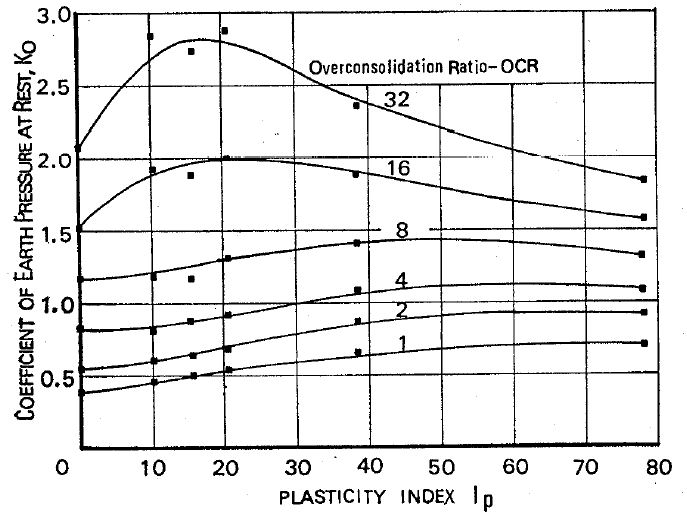
\includegraphics[width=0.9\textwidth]{figures/figure-5.png}
        \caption{Relationship between $K_0$, $I_p$ and OCR}
        \addtocounter{figure}{-1}
        \vspace{-5pt}
        \renewcommand{\figurename}{图}
        \caption{$K_0$,$I_p$和OCR之间的关系\citep{Brooker19651}}
        \renewcommand{\figurename}{Figure}
        \label{figure:5}
    \end{minipage}
    \begin{minipage}[t]{0.42\textwidth}
        \centering
        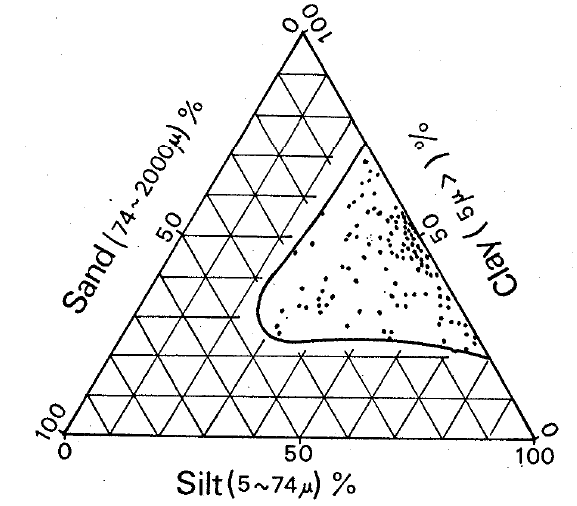
\includegraphics[width=\textwidth]{figures/figure-6.png}
        \caption{Trianguler classification chart}
        \addtocounter{figure}{-1}
        \vspace{-5pt}
        \renewcommand{\figurename}{图}
        \caption{三角分类图}
        \renewcommand{\figurename}{Figure}
        \label{figure:6}
    \end{minipage}
\end{figure*}


\Paragraph{Soil Classification 土体分类}

\begin{paracol}{2}
    
    The data on initial shear modulus, shear strength and N-value of the standard penetration test were obtained from 25 sites, which consisted of 15 alluvial deposits, 9 diluvial deposits, and 1 tertiary deposit.

    In order to describe the physical properties of soils used for this investigation, the triangular classification chart for the results of mechanical analysis is shown in \autoref{figure:6}, the results of plasticity and liquid limit test are shown in \autoref{figure:7} by the plasticity chart, while the relation between overconsolidation ratio and plasticity index are shown in \autoref{figure:8}, and the relation between degree of saturation and void ratio in \autoref{figure:9}.

    \switchcolumn

    标准贯入试验的初始剪切模量,剪切强度和N值的数据来自25个站点,包括15个冲积层,9个冲积层和1个三次层。
   
    为了描述用于该研究的土壤的物理性质,\cnfigureref{figure:6}所示为力学分析结果的三角分类图,塑性图则显示了可塑性和液体极限试验的结果,\cnfigureref{figure:7}所示。 固结率与塑性指标的关系如\cnfigureref{figure:8}所示,饱和度与空隙率的关系如\cnfigureref{figure:9}所示。

\end{paracol}

\begin{figure*}[!htb]
    \begin{minipage}[t]{0.32\textwidth}
        \centering
        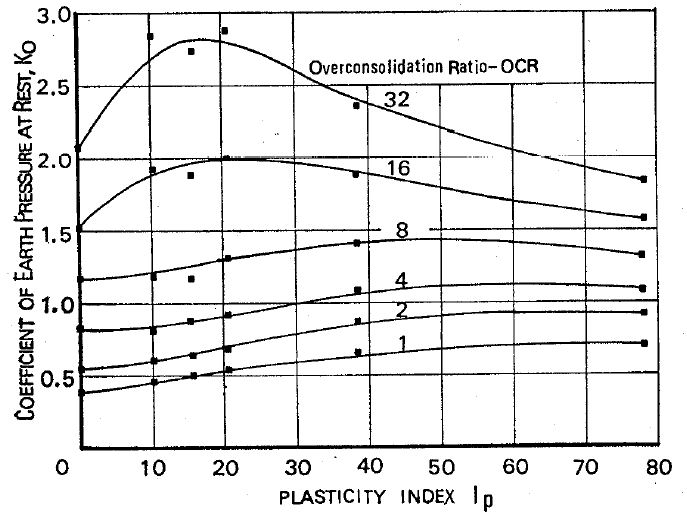
\includegraphics[width=\textwidth]{figures/figure-5.png}
        \caption{Relationship between $I_p$ and $W_L$}
        \addtocounter{figure}{-1}
        \vspace{-5pt}
        \renewcommand{\figurename}{图}
        \caption{$I_p$和$W_L$之间的关系\citep{Brooker19651}}
        \renewcommand{\figurename}{Figure}
        \label{figure:7}
    \end{minipage}
    \begin{minipage}[t]{0.32\textwidth}
        \centering
        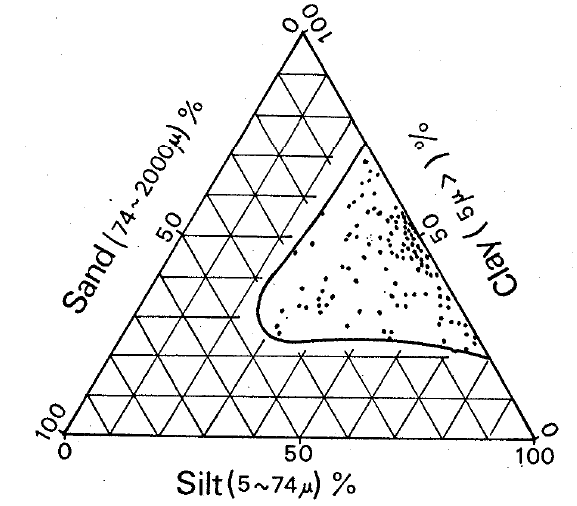
\includegraphics[width=\textwidth]{figures/figure-6.png}
        \caption{Relationship between OCR and $I_p$}
        \addtocounter{figure}{-1}
        \vspace{-5pt}
        \renewcommand{\figurename}{图}
        \caption{OCR和$I_p$之间的关系}
        \renewcommand{\figurename}{Figure}
        \label{figure:8}
    \end{minipage}
    \begin{minipage}[t]{0.32\textwidth}
        \centering
        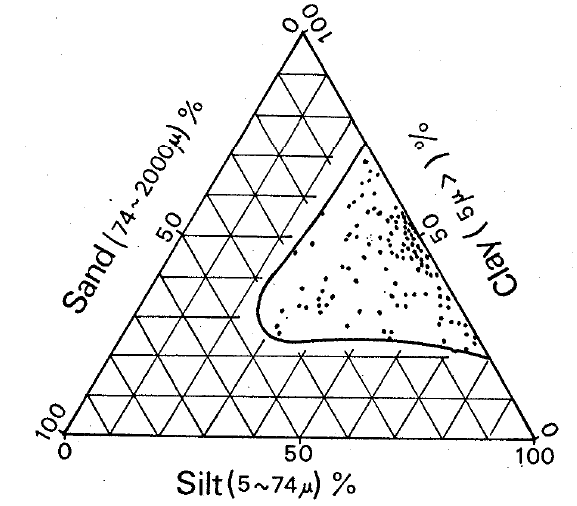
\includegraphics[width=\textwidth]{figures/figure-6.png}
        \caption{Relationship between $S_r$ and $e$}
        \addtocounter{figure}{-1}
        \vspace{-5pt}
        \renewcommand{\figurename}{图}
        \caption{$S_r$和$e$之间的关系}
        \renewcommand{\figurename}{Figure}
        \label{figure:9}
    \end{minipage}
\end{figure*}


\begin{paracol}{2}
    
    The physical properties of the soil used in this paper are summarized as follows from \autoref{figure:6}, \autoref{figure:7}, \autoref{figure:8} and \autoref{figure:9}: 

    \begin{enumerate}
        \item Soil belongs to the category of cohesive soil.
        \item The plasticity index has a wide range of distribution.
        \item The values of overconsolidation ratio range from 1.0 to 3.0.
        \item The values of void ratio range from 0.5 to 3.0, and most of the data are from 1.0 to 2.0.
        \item The values of the degree of saturation range from 90$\%$ to 100$\%$, and most of the data nearly 100$\%$.
    \end{enumerate}

    \switchcolumn

    \cnfigureref{figure:6},\cnfigureref{figure:7},\cnfigureref{figure:8}和\cnfigureref{figure:9}总结了本文使用的土壤的物理特性:
    \begin{enumerate}
        \item 土体属于黏性土。
        \item 可塑性指数分布范围广。
        \item 超固结比的值范围为1.0至3.0。
        \item 空隙率的值范围为0.5至3.0,大多数为1.0至2.0。
        \item 饱和度的值范围从90$\%$到100$\%$,大多数接近100$\%$。
    \end{enumerate}

\end{paracol}
\section{INITIAL SHEAR MODULUS AND N-VALUE 初始剪切模量和N值}

\begin{paracol}{2}
    
    The well-shooting test is gradually being adopted widely , because it is proven to be provided with such advantageous features that : 
    \begin{enumerate}
        \item eimmate any necessity o securing an extensive area for measurement;
        \item ensure higher accuracy of measurement, compared with surface refraction method;
        \item allow wave velocity measurement in a soft soil layer, even if there exists a hard layer above it.
    \end{enumerate}

    \switchcolumn

    地震测井试验试验正逐渐被广泛采用,因为事实证明它具有以下优点:
    \begin{enumerate}
        \item 消除了任何必要,确保了广阔的测量范围;
        \item 与表面折射法相比,确保更高的测量精度;
        \item 即使在软土层之上,也可以进行波速测量。
    \end{enumerate}

    \switchcolumn*

    A review of the data on the well-shooting tests conducted in the past has led the authors to take notice that there have been a number of instances where the well-shooting test and the standard penetration test were conducted on the same site. It is therefore necessary to make an investigation into the relationship between the shear modulus and the N-value of soil deposits obtained respectively by the well-shooting test and the standard penetration test, so as to get a better knowledge of elastic properties of soil. When the value of initial shear modulus and N-value are to be sampled from the existing data, it is necessary, however, to set up certain criteria to avoid any partial data sampling.

    \switchcolumn

    对过去进行的地震测井试验数据的回顾使作者注意到,在许多情况下,在同一地点进行了地震测井试验和标准贯入试验。 因此,有必要对分别通过地震测井试验和标准贯入试验获得的土壤沉积物的剪切模量与N值之间的关系进行研究,以便更好地了解土壤的弹性。 但是,当要从现有数据中采样初始剪切模量和N值时,有必要设置某些标准以避免任何部分数据采样。

\end{paracol}

\Paragraph{Criteria of Data Sampling 数据采样标准}

\begin{paracol}{2}

    In the case of the authors' investigation, criteria of data sampling were set up so that such data as might meet the following requirements could only be adopted :

    \switchcolumn

    在作者调查的情况下,建立数据采样标准,以便只能采用可能满足以下要求的数据:

    \switchcolumn*

    \begin{enumerate}
        \item Soil has to fall under the category of cohesive soil.
        \item Shear wave velocity has to be measured by way of the well-shooting test.
        \item Uniform section of shear wave velocity values and N-values has to be more than 2.0 m, as shown in \autoref{figure:10} "An Example of Data Sampling."
        \item The well-shooting test and the standard penetration test have to be conducted on the same site.
    \end{enumerate}

    \switchcolumn
    \begin{enumerate}
        \item 土体必须属于黏性土体。
        \item 剪切波速度必须通过地震测井试验来测量。
        \item 剪切波速度值和N值的均匀截面必须大于2.0 m,如\cnfigureref{figure:10}“数据采样示例”所示。
        \item 地震测井试验和标准贯入试验必须在同一地点进行。
    \end{enumerate}
    
\end{paracol}

\begin{figure*}[!htb]
    \begin{minipage}[t]{0.50\textwidth}
        \centering
        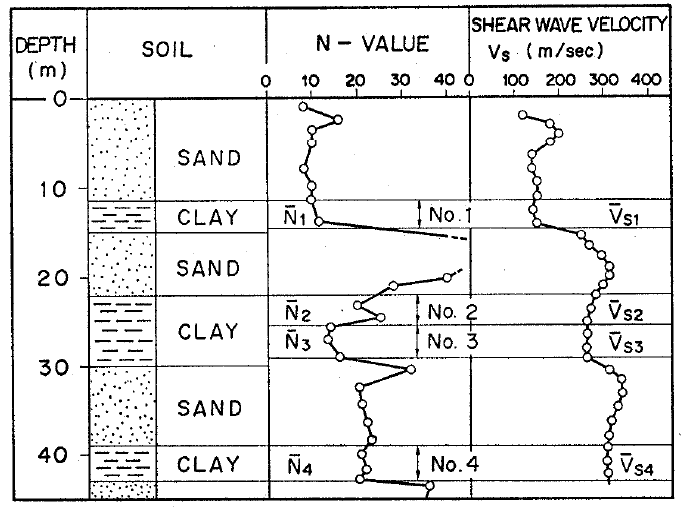
\includegraphics[width=\textwidth]{figures/figure-10.png}
        \caption{An example of data sampling}
        \addtocounter{figure}{-1}
        \vspace{-5pt}
        \renewcommand{\figurename}{图}
        \caption{数据采样示例}
        \renewcommand{\figurename}{Figure}
        \label{figure:10}
    \end{minipage}
    \begin{minipage}[t]{0.46\textwidth}
        \centering
        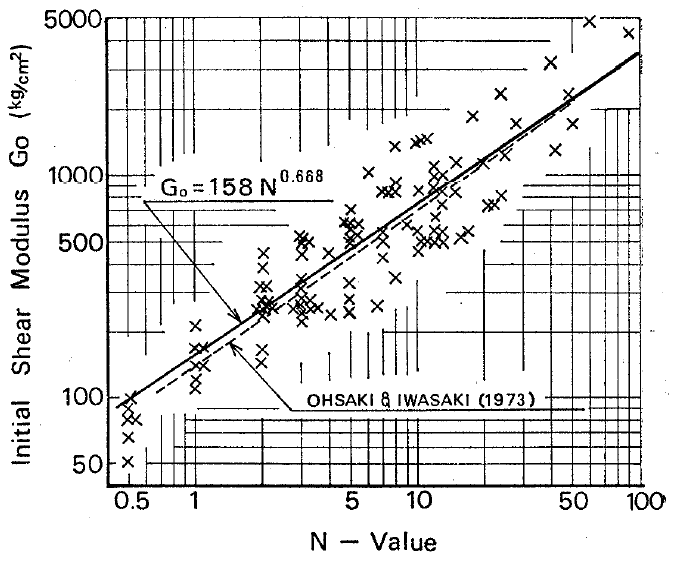
\includegraphics[width=\textwidth]{figures/figure-11.png}
        \caption{Relationship between $G_0$ and N-value}
        \addtocounter{figure}{-1}
        \vspace{-5pt}
        \renewcommand{\figurename}{图}
        \caption{$G_0$和N值之间的关系}
        \renewcommand{\figurename}{Figure}
        \label{figure:11}
    \end{minipage}
\end{figure*}

\Paragraph{Relation between Initial Shear Modulus and N-Value 初始剪切模量与N值之间的关系}

\begin{paracol}{2}
    
    The data on initial shear modulus $G_0$ and N-value thus sampled in conformity with the above criteria of data sampling are plotted on a logarithmic graph as shown in \autoref{figure:11}. \autoref{figure:11} shows that $G_0$ and N-value is in approximate proportion to each other on the logarithmic graph.

    Accordingly, on the assumption that the first order equation should be $G_0=aN^b$ the following empirical formula was obtained by calculating $a$ and $b$ by the least squares method :

    \switchcolumn

    这样按照上述数据采样标准采样的初始剪切模量$G_0$和N值的数据绘制在对数图上,如\cnfigureref{figure:11}所示。图\cnfigureref{figure:11}表明,$G_0$和N值与比例大致成比例。 在对数图中彼此。
       
    因此,假设一阶方程应为$G_0=aN^b$,则通过最小二乘法计算$a$和$b$可获得以下经验公式: 

\end{paracol}

\begin{align}
    G_0=158N^{0.668}(\rm{kg/cm^2})
    \label{equation:9}
\end{align}

\begin{paracol}{2}
    
    \noindent{}where coefficient of correlation $\rho_{xy}=0.88$. 

    \switchcolumn

    \noindent{}其中相关系数$\rho_{xy}=0.88$。

\end{paracol}

\Paragraph{Comparison with Other Investigations 与其他调查研究的比较}

\begin{paracol}{2}
    
    Ohsaki and Iwasaki have evaluated the relation between $G_0$ and N-value by arranging the data obtained from well-shooting tests and standard penetration tests, which were collected by the Evaluation Committee on High-Rise Building Structures, the Building Center of Japan. With classification of soil into cohesive soil and sandy soil with a view to facilitating evaluation of the relation between $G_0$ and N-value, they have shown for cohesive soils that the following empirical formula existed between $G_0$ and N-value:

    \switchcolumn

    \citet{Ohsaki197361}通过安排由日本建筑中心高层建筑结构评估委员会收集的地震测井试验和标准贯入试验获得的数据,评估了$G_0$和N值之间的关系。为了便于评估$G_0$和N值之间的关系,将土壤分为黏性土和砂土,他们表明对于黏性土,在$G_0$和N值之间存在以下经验公式:

\end{paracol}

\begin{align}
    G_0=140N^{0.722}(\rm{kg/cm^2})
    \label{equation:10}
\end{align}

\begin{paracol}{2}
    
    \noindent{}where coefficient of correlation $\rho_{xy}=0.90$. Graphical expression of \autoref{equation:9} and \autoref{equation:10} show that there is quite a similarity between them, as illustrated in Fig. 11.

    \switchcolumn

    \noindent{}其中相关系数$\rho_{xy}=0.90$。 \cnequationref{equation:9}和\cnequationref{equation:10}的图形表明,它们之间有相当的相似性,如\cnfigureref{figure:11}所示。
\end{paracol}
\section*{SHEAR STRENGTH AND N-VALUE 抗剪强度和N值}

\begin{paracol}{2}
    
    Now that the relation between shear modulus $G_0$ and N-value of the standard penetration test has been evaluated in the preceding section, the relation between shear strength $S_u$ and N-value has to be evaluated, too, in a similar way.

    Shear strength $S_u$ can be obtained from \autoref{equation:8} by use of the results of triaxial compression test on undisturbed soil samples. When the relation between shear strength and N-value is to be evaluated, particular attention has to be paid to soil sampling practice and accuracy of soil test. With this taken into account, the authors have sampled data solely from such basic soil exploration reports as considered to be under stringent supervision for securing as high accuracy as possible of soil test and, especially, the results of such soil tests as were conducted with special attention paid to sampling method\citep{Koizumi1968} or by use of block samples, since soil samples are easy to be disturbed, if N-value exceeds 10.

    \switchcolumn

    现在,在上一节中已经评估了剪切模量$G_0$与标准渗透试验的N值之间的关系,因此也必须以类似的方式评估剪切强度$S_u$与N值之间的关系。
        
    抗剪强度$S_u$可以使用\cnequationref{equation:8}的三轴压缩试验结果在未经扰动的土体样品上获得。 当要评估抗剪强度与N值之间的关系时,必须特别注意土体取样和土体试验的准确性。 考虑到这一点,作者仅从基本的土体勘探报告中取样数据,这些报告被认为受到严格的监督,以确保尽可能高的土体测试准确性,尤其是在特殊条件下进行的土体测试结果 注意如果N值超过10,土体样本很容易受到干扰,请注意抽样方法\citep{Koizumi1968}或使用块状样本。

\end{paracol}

\Paragraph{Criteria of Data Sampling 数据采样标准}

\begin{paracol}{2}
    
    Criteria of data sampling was set up so that the following requirements could be satisfied :
    \begin{enumerate}
        \item Soil has to fall under the category of cohesive soil.
        \item Soil sampling and standard penetration test have to be carried out in the same borehole.
        \item Any data with N-value of less than 1.0 shall be rejected, because there exists no coefficient of correlation between shear strength and N-value, if the latter is less than 1.0.
    \end{enumerate}
    \switchcolumn

    建立了数据采样标准,以便满足以下要求:
    \begin{enumerate}
        \item 土样必须属于黏性土体。
        \item 必须在同一钻孔中进行土体取样和标准渗透试验。
        \item 任何N值小于1.0的数据均应被拒绝,因为如果N值小于1.0,则抗剪强度与N值之间不存在相关系数。
    \end{enumerate}
    
\end{paracol}

\Paragraph{Relation between Shear Strength and N-Value 抗剪强度与N值的关系}

\begin{paracol}{2}
    
    Just as in the preceding section, the data on shear strength and N-value thus sampled are plotted on a logarithmic graph shown in \autoref{figure:12}. On the assumption that the first order equation should be $S_u=aN^b$, the following empirical formula was obtained by calculating $a$ and $b$ the method of least squares :

    \switchcolumn

    与前面的部分一样,将这样取样的抗剪强度和N值数据绘制在\cnfigureref{figure:12}所示的对数图上。假设一阶方程应为$S_u=aN^b$,则可通过以下公式获得以下经验公式:计算$a$和$b$的最小二乘法:

\end{paracol}

\begin{align}
    S_u=0.297N^{0.72}(\rm{kg/cm^2})
    \label{equation:11}
\end{align}
\begin{figure*}[!htb]
    \begin{minipage}[t]{0.48\textwidth}
        \centering
        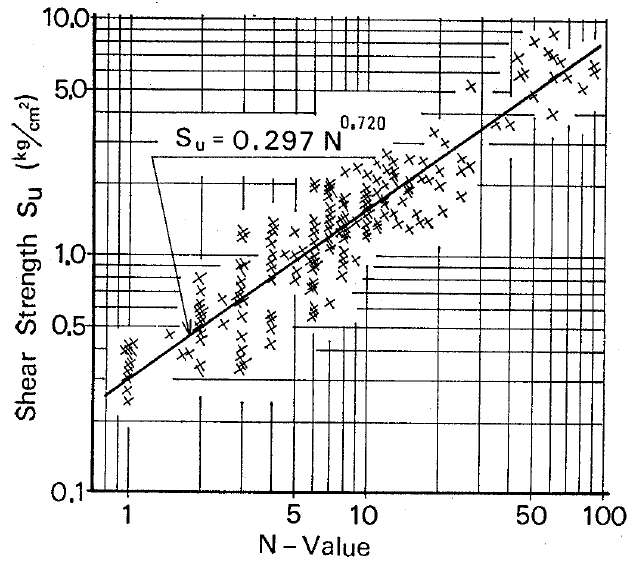
\includegraphics[width=\textwidth]{figures/figure-12.png}
        \caption{Relationship between $S_u$ and N-value}
        \addtocounter{figure}{-1}
        \vspace{-5pt}
        \renewcommand{\figurename}{图}
        \caption{$S_u$和N值之间的关系}
        \renewcommand{\figurename}{Figure}
        \label{figure:12}
    \end{minipage}
    \begin{minipage}[t]{0.48\textwidth}
        \centering
        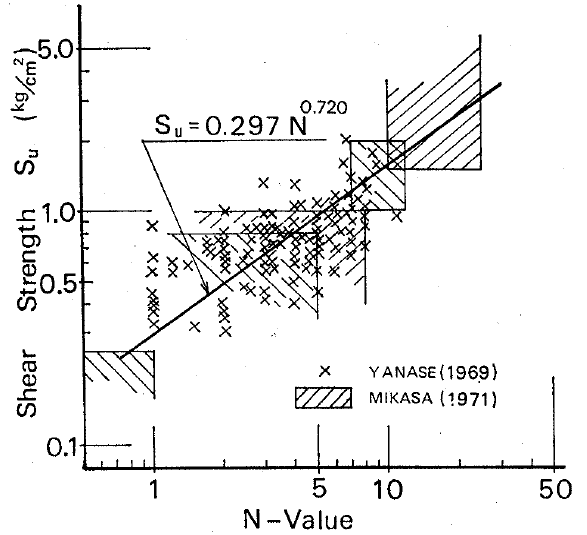
\includegraphics[width=\textwidth]{figures/figure-13.png}
        \caption{Comparison between \autoref{equation:11} and similar data by others}
        \addtocounter{figure}{-1}
        \vspace{-5pt}
        \renewcommand{\figurename}{图}
        \caption{\autoref{equation:11}与其他类似数据之间的比较}
        \renewcommand{\figurename}{Figure}
        \label{figure:13}
    \end{minipage}
\end{figure*}


\begin{paracol}{2}

    \noindent{}where coefficient of correlation $\rho_{xy}=0.93$.

    \switchcolumn      
     
    \noindent{}其中相关系数$\rho_{xy}=0.93$。

\end{paracol}

\Paragraph{Comparison with Other Investigations 与其他调查研究的比较}

\begin{paracol}{2}
    

    The shear strength of clay can be approximately obtained from the unconfined compression strength $q_u$ by the following equation.

    \switchcolumn

    黏土的剪切强度可以通过以下等式从无侧限抗压强度$q_u$近似获得。

\end{paracol}

\begin{align}
    S_u\doteq\frac{1}{2}q_u(\rm{kg/m^2})
\end{align}

\begin{paracol}{2}

    \citet{Mikasa197138} has shown the range of N-value and unconfined compression strength of cohesive soil on the basis of his investigation into typical cohesive soil layers in Osaka district. Similarly, \citet{Yanase196937} has shown many data on N-value and unconfined compression strength of cohesive soil by way of his test conducted on such soil samples as considered to have been least disturbed during sampling. These data are plotted in \autoref{figure:13} together with graphical expression of \autoref{equation:11}, which is expressed as a straight line passing near the center of those data shown by Mikasa\citet{Mikasa197138} and Yanase\citet{Yanase196937}.

    \switchcolumn

    \citet{Mikasa197138}在对大阪地区典型的黏性土层进行调查的基础上,显示了黏性土的N值范围和无侧限抗压强度。 同样,\citet{Yanase196937}通过对这样的土壤样本进行的测试,显示出许多关于黏性土壤的N值和无侧限抗压强度的数据,这些样本被认为在采样过程中受到的干扰最小。 这些数据与\cnequationref{equation:11}的图形表达式一起绘制在\cnfigureref{figure:13}中,该等式表示为一条直线,通过的直线靠近Mikasa\citet{Mikasa197138}和Yanase\citet{Yanase196937}展示的那些数据的中心。

\end{paracol}
\section{INITIAL SHEAR MODULUS AND SHEAR STRENGTH 初始剪切模量和剪切强度}

\begin{paracol}{2}
    
    So far, the authors'effort has been directed toward evaluating relationship between N-value of the standard penetration test and initial shear modulus or shear strength of cohesive soil.
    
    In this section, however, their effort is to be directed solely to evaluating direct relation between initial shear modulus $G_0$ and shear strength $S_u$. It is to be noted here that criteria of data sampling can be more moderate in this section, because of reduction in number of data on initial shear modulus and N-value, compared with the previous sections.
    
    The data for use in this section are from one of the investigations made in the past by other researchers\citet{Shima19681301, Shima1969819} and such data sources as Kajima Institute of Construction Technology by which the authors are employed, involving 20 sites and 194 data in total.

    \switchcolumn

    到目前为止,作者一直致力于评估标准渗透试验的N值与粘性土的初始剪切模量或剪切强度之间的关系。
            
    然而,在本节中,他们的工作将仅针对评估初始剪切模量$G_0$与剪切强度$S_u$之间的直接关系。 这里要注意的是,与之前的部分相比,由于初始剪切模量和N值的数据数量减少,本部分中的数据采样标准可能更为温和。
            
    本节中使用的数据来自于其他研究人员\citet{Shima19681301, Shima1969819}过去的一项调查,以及来自作者的鹿岛建设技术研究所等数据源,涉及20个地点,共194个数据。
    
\end{paracol}

\Paragraph{Criteria of Data Sampling 数据采样标准}

\begin{paracol}{2}

    Criteria of Data Sampling Criteria of data sampling was set up so that the following requirements could be met : 
    \begin{enumerate}
        \item Soil has to fall under the category of cohesive soil.
        \item Shear wave velocity has to be measured by way of the well- shooting test.
        \item Values of $G_0$ and $S_u$ have to be those obtained by experiment at the same site and in the same depth. If there exist several values for $S_u$ corresponding number of data should be made availably by combining each value of $S_u$ with the corresponding value of $G_0$.
    \end{enumerate}

    \switchcolumn

    数据采样标准设置数据采样标准是为了满足以下要求:
    \begin{enumerate}
        \item 土体必须属于黏性土体。
        \item 剪切波速度必须通过射井试验来测量。
        \item $G_0$和$S_u$的值必须是在相同的位置和相同的深度通过实验获得的。 如果存在$S_u$的多个值,则应通过将$S_u$的每个值与$G_0$的对应值进行组合来获得对应数量的数据。
    \end{enumerate}
    
\end{paracol}

\Paragraph{Relation between Initial Shear Modulus and Shear Strength 初始剪切模量与剪切强度之间的关系}

\begin{paracol}{2}
    
    Data on initial shear modulus $G_0$ and shear strength $S_u$ are plotted on a logarithmic graph shown in \autoref{figure:14}. On the assumption that as a first approximation equation should be $G_0=aS_u^b$ and taking the data plotted in \autoref{figure:14} into account, the following empirical formula was obtained by calculating a and b by the method of least squares :

    \switchcolumn

    初始剪切模量$G_0$和抗剪强度$S_u$的数据绘制在\cnfigureref{figure:14}所示的对数图上。假设作为第一近似方程式,应为$G_0=aS_u^b$,并考虑\cnfigureref{figure:14}中绘制的数据, 通过最小二乘法计算$a$和$b$得到以下经验公式:

\end{paracol}

\begin{align}
    G_0=516S_u^{1.012}(\rm{kg/m^2})
    \label{equation:13}
\end{align}

\begin{figure*}[!htb]
    \begin{minipage}[t]{0.44\textwidth}
        \centering
        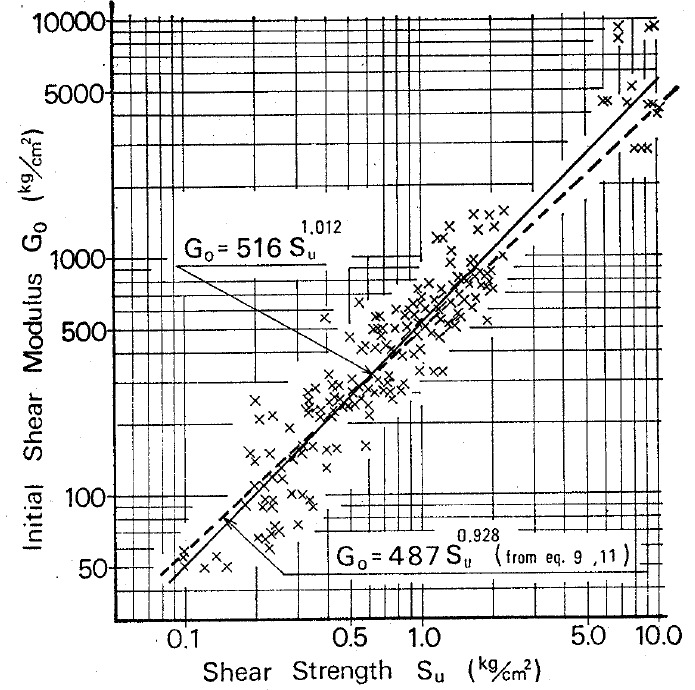
\includegraphics[width=\textwidth]{figures/figure-14.png}
        \caption{Relationship between $G_0$ and $S_u$}
        \addtocounter{figure}{-1}
        \vspace{-5pt}
        \renewcommand{\figurename}{图}
        \caption{$G_0$和$S_u$值之间的关系}
        \renewcommand{\figurename}{Figure}
        \label{figure:14}
    \end{minipage}
    \begin{minipage}[t]{0.52\textwidth}
        \centering
        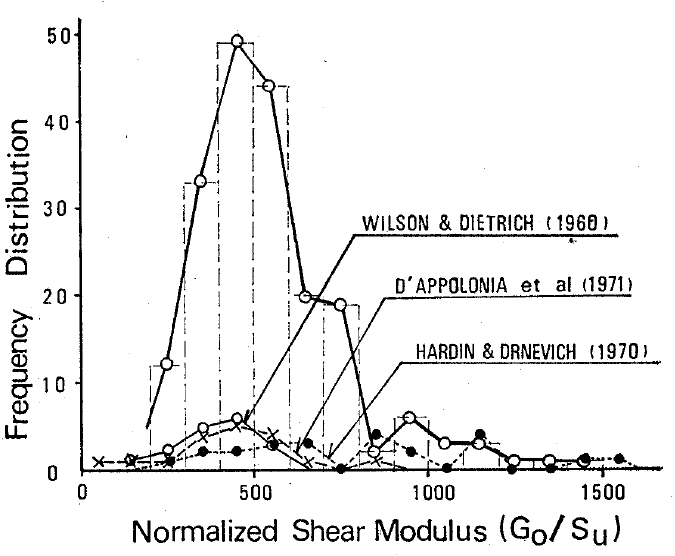
\includegraphics[width=\textwidth]{figures/figure-15.png}
        \caption{Histogram of normalized shear modulus ($G_0/S_u$)}
        \addtocounter{figure}{-1}
        \vspace{-5pt}
        \renewcommand{\figurename}{图}
        \caption{归一化剪切模量的直方图($G_0/S_u$)}
        \renewcommand{\figurename}{Figure}
        \label{figure:15}
    \end{minipage}
\end{figure*}


\begin{paracol}{2}

    \noindent{}where coefficient of correlation $\rho_{xy}=0.95$.

    \switchcolumn
    
    \noindent{}其中相关系数$\rho_{xy}=0.95$。

    \switchcolumn*

    Exponent of $S_u$ in the \autoref{equation:13} is 1.012 or approximately equal to 1.0. $G_0$ can therefore be considered to be in proportion to $S_u$.

    \switchcolumn

    $S_u$在\cnequationref{equation:13}中的指数为1.012或大约等于1.0。 因此,可以认为$G_0$与$S_u$成比例。

\end{paracol}

\Paragraph{Investigation of Normalized Shear Modulus 归一化剪切模量的研究}

\begin{paracol}{2}
    
    Now that $G_0$ is confirmed to be in proportion to $S_u$, it is convenient to define the normalized shear modulus $G_n$ as follows :

    \switchcolumn

    既然已确定$G_0$与$_Su$成比例,则可以方便地将归一化剪切模量$G_n$定义如下:

\end{paracol}

\begin{align}
    G_n=\frac{G_0}{S_u}
    \label{equation:14}
\end{align}

\begin{paracol}{2}
    
    \autoref{figure:14} shows a histogram of the normalized shear modulus drawn by calculating values of $G_n$ from the data plotted in \autoref{figure:14}. The value of $G_n$ are in the region ranging from 250 to 1430, with the mean value of 548 and the standard deviation of 211.
    
    For comparison, the following values of $G_n$ can be quoted independently from the data obtained by \citet{Hardin1973667}, \citet{Wilson2010419} and \citet{DAppolonia19711359}.

    \switchcolumn

    \cnfigureref{figure:15}显示了通过从\cnfigureref{figure:14}中绘制的数据计算$G_n$值得出的归一化剪切模量的直方图。$G_n$值在250到1430的范围内,平均值为548,标准偏差为211。
    
    为了比较,可以独立于由\citet{Hardin1973667},\citet{Wilson2010419}和\citet{DAppolonia19711359}获得的数据引用的以下$G_n$值。

    \switchcolumn*
    
    \begin{enumerate}
        \item \citet{Hardin1973667} have obtained the initial shear modulus and the shear strength of the same cohesive soil by means of a reasonant-column apparatus in the laboratory. The normalized shear modulus $G_n$ calculated from these values is ranging from 380 to 1500 with its mean value of about 760.
        \item \citet{Wilson2010419} have obtained the values of initial Young's modulus, initial shear modulus and compressible strength by measuring a -longitudinal or torsional natural frequency of clay samples. The value of $G_n$ can be calculated from these measured data by assumming the Poisson's ratio as 0.5, and it is in the region ranging from 178 to 550 with its mean value of about 390.
        \item \citet{DAppolonia19711359} have shown eleven combinations of data on the initial Young's modulus and the shear strength by in-situ and laboratory tests. 
    \end{enumerate}      

    \switchcolumn
    
    \begin{enumerate}         
        \item \citet{Hardin1973667}通过实验室中的推理柱设备获得了同一粘性土的初始剪切模量和剪切强度。 根据这些值计算出的归一化剪切模量$G_n$介于380至1500之间,其平均值约为760。
        \item \citet{Wilson2010419}通过测量粘土样品的纵向或扭转自然频率获得了初始杨氏模量,初始剪切模量和可压缩强度的值。 可以通过将泊松比设为0.5来从这些测量数据中计算出$G_n$值,该值处于178至550范围内,平均值约为390。
        \item \citet{DAppolonia19711359}通过现场和实验室测试,已显示出有关初始杨氏模量和剪切强度的11种数据组合。
    \end{enumerate}

    \switchcolumn*
    
    The value of $G_n$ calculated from these values by assumming the Poisson's ratio as 0.5 is in the region ranging from 53 to 833 with its mean value about 420. 
    
    The results of these investigations are shown in \autoref{figure:15} for comparison with the authors' result. The histogram in \autoref{figure:15} shows that the peaks of frequency distribution curves are in the region ranging from 400 to 500 except \citet{Hardin1973667}'s data.

    \switchcolumn
       
    通过假设泊松比为0.5,从这些值计算出的$G_n$值在53到833范围内,其平均值约为420。
       
    这些研究的结果如\cnfigureref{figure:15}所示,以便与作者进行比较。\cnfigureref{figure:15}的直方图显示,除\citet{Hardin1973667}的数据外,频率分布曲线的峰值在400到500范围内。
    
\end{paracol}
\section*{DISCUSSION AND CONCLUSIONS 讨论和结论}

\begin{paracol}{2}
    
    The standard penetration test is easy and less expensive to conduct mainly because of its standardization, though it has a drawback in rather low accuracy. Investigation into soil deposits by way of the standard penetration test allows a three-dimensional grasp of their structure, if the test is conducted as many times as possible, so that as many test data as possible can be obtained.

    \switchcolumn

    标准渗透测试容易进行且成本较低,这主要是由于其标准化,尽管它具有准确性较低的缺点。 通过标准渗透试验对土壤沉积物进行调查,可以对结构进行三维掌握,如果该试验进行了尽可能多的次数,则可以获得尽可能多的试验数据。  
    
    \switchcolumn*

    With due attention paid to such advantageous feature of the standard penetration test, the authors have finally succeeded in introducing \autoref{equation:9} and \autoref{equation:11} by arranging in a statistical way the data on initial shear modulus $G_0$, shear strength $S_u$ and N-value of the standard penetration test.
    
    \switchcolumn
       
    在充分注意标准渗透试验的这种有利特性的基础上,作者们终于成功地引入了\cnequationref{equation:9}和\cnequationref{equation:11},通过统计方式安排了初始剪切模量$G_0$,剪切强度$S_u$和N值的数据。 标准渗透测试。      
    \switchcolumn*

    On the other hand, the authors have also evaluated the relation between $G_0$ and $S_u$, so that it turns out to be expressed in \autoref{equation:13}. Elimination of N from the \autoref{equation:9} and \autoref{equation:11} allows the relation between $G_0$ and $S_u$ to be expressed in the following equation :

    \switchcolumn
       
    另一方面,作者还评估了$G_0$和$S_u$之间的关系,从而证明它由\cnequationref{equation:13}表示。 从等式\cnequationref{equation:9}和\cnequationref{equation:11}消除N可以使$G_0$和$S_u$之间的关系表示为以下方程式: 

\end{paracol}

\begin{align}
    G_0=487S_u^{0.928}(\rm{kg/m^2})
    \label{equation:15}
\end{align}

\begin{paracol}{2}

    \autoref{equation:15} is represented in \autoref{figure:14}, so that it can be compared with \autoref{equation:13}. A close resemblance existing between the two equations is self-explanatory of mutual relationship among initial shear modulus, shear strength and N-value.

    The investigations covered in this paper are summarized as follows.

    \switchcolumn

    \cnequationref{equation:15}在\cnfigureref{figure:14}中表示,因此可以将其与\cnequationref{equation:13}进行比较。 这两个方程之间存在非常相似的地方,这很容易说明初始剪切模量,剪切强度和N值之间的相互关系。
    本文涵盖的研究概述如下。

    \switchcolumn*

    \begin{enumerate}
        \item Shear strain amplitude generated in a very soft soil deposit by the well-shooting test was in general found less than $10^{-3}\%$. It follows from this that shear modulus obtained by in-situ tests can be regarded as the initial shear modulus.
        \item As a result of investigating the mutual relationship among initial shear modulus, shear strength and N-value, it became clear that the initial shear modulus of cohesive soil is proportional to its shear strength obtained under the $K_0$-condition.
        \item The ratio between the initial shear modulus and the shear strength can be estimated to be about 500 from \autoref{equation:13}and \autoref{figure:15}.
        \item It is simple and convenient if the initial shear modulus is estimated from N-value. However, we should not resort to N-value only, because errors of the standard penetration test become large, especially when N-value is less than 2.
    \end{enumerate}
    
    \switchcolumn

    \begin{enumerate}
        \item 一般情况下,通过射孔试验在非常软的土壤沉积物中产生的剪切应变振幅通常小于$10^{-3}\%$。 由此可知,可以将通过原位测试获得的剪切模量视为初始剪切模量。
        \item 研究了初始剪切模量,剪切强度和N值之间的相互关系,结果发现,黏性土的初始剪切模量与其在$K_0$条件下获得的剪切强度成正比。
        \item 根据\cnequationref{equation:13}和\cnfigureref{figure:15}可以估计出初始剪切模量与剪切强度之间的比率约为500。
        \item 如果根据N值估算初始剪切模量,则既简单又方便。 但是,我们不应仅诉诸N值,因为标准渗透测试的误差会变得很大,尤其是当N值小于2时。
    \end{enumerate}

\end{paracol}
\section*{ACKNOWLEDGEMENT 致谢}

\begin{paracol}{2}
    
    The authors wish to express their gratitude to Dr. Y. Ohsaki, Professor of University of Tokyo, and Dr. H. Kishida, Associate Professor of Tokyo Institute of Technology · for their kind guidance and encouragement.

    \switchcolumn

    作者谨向东京大学教授Dr. Y. Ohsaki和东京工业大学副教授Dr. H. Kishida表示感谢,感谢他们的指导和鼓励。

\end{paracol}

\bibliographystyle{plainnat} % gbt7714-author-year gbt7714-numerical
\bibliography{Hara19741.bib}

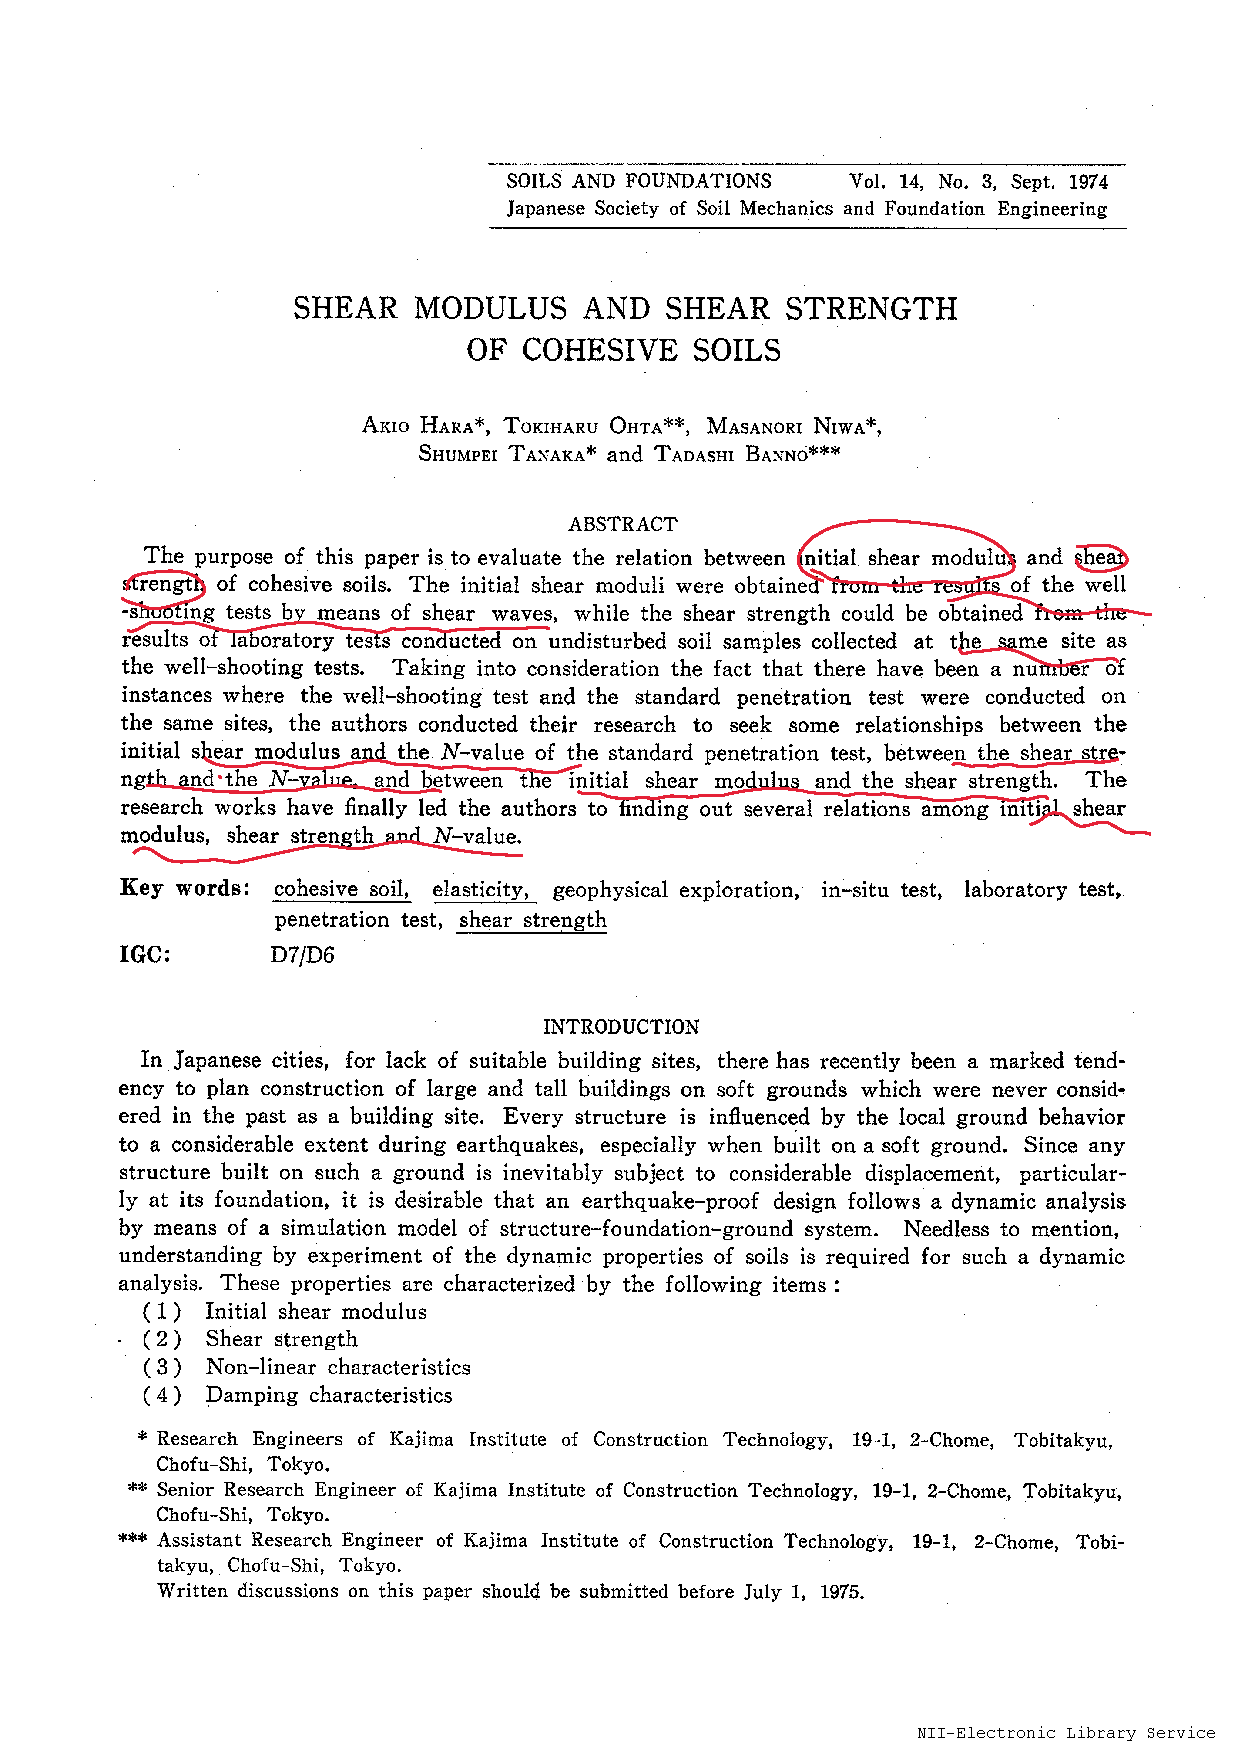
\includepdf[pages=1-12]{Hara 1974 - Shear modulus and shear shear strength of cohesive soils.pdf}

\end{document}